\documentclass{article}
\usepackage{graphicx}
\usepackage[margin=1in]{geometry}
\usepackage{indentfirst}

\begin{document}
\title{Requirements Specification Document}
\author{Team D}
\date{\today}

\maketitle

\vspace*{3.5in}
\begin{table}[htbp]
\caption{Team}
\begin{center}
\begin{tabular}{|r | c|}
\hline
Name & ID Number \\
\hline\hline
Stefanie Lavoie & 1951750 \\
Pinsonn Laverdure & 9684352 \\
Ghislain Ledoux & 6376320 \\
Rigil Malubay & 6262732 \\
Philippe Milot & 9164111 \\
Christopher Mukherjee & 6291929 \\
\hline
\end{tabular}
\end{center}
\end{table}

\pagenumbering{gobble}% Remove page numbers (and reset to 1)
\clearpage

\tableofcontents
\clearpage

\pagenumbering{arabic}% Arabic page numbers (and reset to 1)

\section{Introduction} % Status: Complete

This document will describe in detail the architecture specifications for the Vessel Monitoring System which is to be developed in the context of the COMP354 course. This design document include a detailed version of the architecture design pattern, a 4+1 Architectural View diagram (as well as a description of the rationale of this design), Module Interface Specifications for each subsystem, a complete description of the design of the system and of all its subsystems, full dynamic design scenarios of two substantial use cases, and a revised cost estimation and project schedule.

\section{Architectural Design} % Status: See subsections

\subsection{Architecture Diagram} % Status: See subsubsections
Previously in the program, we had the main method calling the information on a timer and sending the information to the GUI. 
This approach caused the entire system (including all subsystems) to execute synchronously, making the VMS dependent on the implementation details of the vessel simulator.
We reworked the architecture of the program and now it is separated into several subsystems.
All of these subsystems now work and involve independently from each other.
\subsubsection{Logical View} % Status: Complete
\begin{figure}[!htb]
\caption{Communication Diagram of the Simulator Subsystem}
\centering
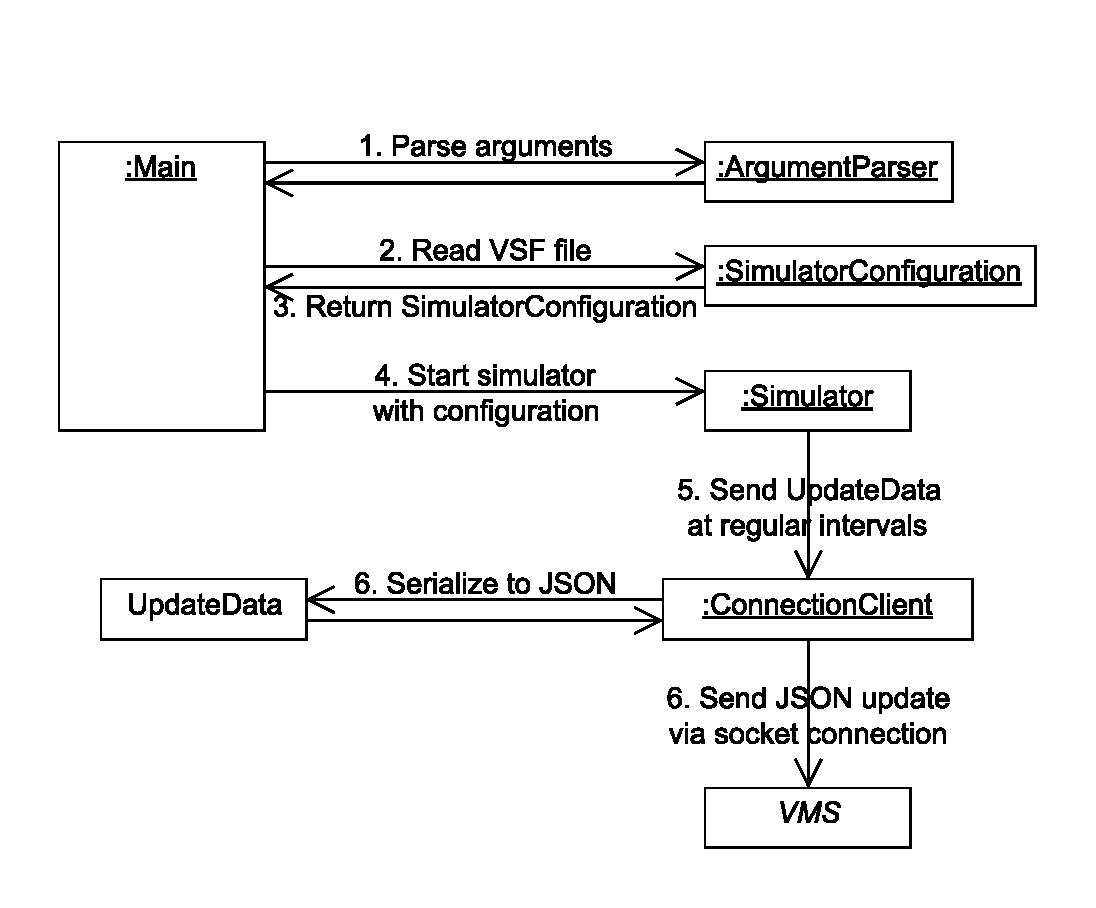
\includegraphics[scale=0.7]{diagrams/simulator-communication-diagram.eps}
\end{figure}
When the program is started, this subsystem will start and parse the arguments that are given to it. Following that it will read from the vsf file from which it will create a simulatorConfiguration instance. With the configuration created from the vsf file, it will start the simulator. At regular intervals, the simulator will generate an UpdateData from the VSF information and send it to the VMS server using the ConnectionClient class.

\break
\begin{figure}[!htb]
\caption{Class Diagram of the Simulator Subsystem}
\centering
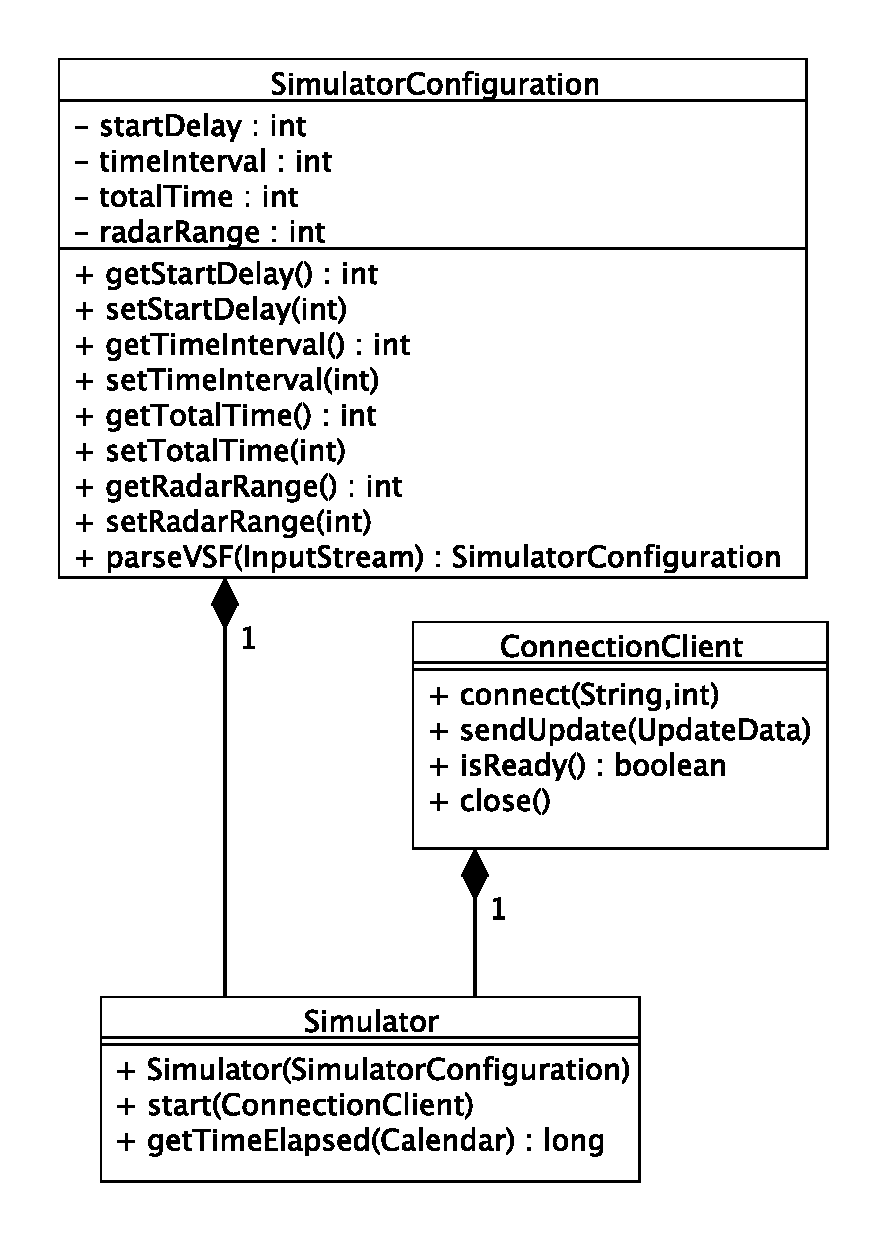
\includegraphics[scale=0.7]{diagrams/simulator-class-diagram.eps}
\end{figure}
These are the classes involved in the configuration process of the creation of the simulator. As stated for Figure 1, simulatorConfiguration class will take on a vsf file for it to parse, with that it will ensure that the configuration is valid. The ConnectionClient abstracts away the details of sending an UpdateData over the network to the VMS. The Simulator aggregates these two classes in order to send UpdateData instances to the VMS at regular intervals.

\break
\begin{figure}[!htb]	
\caption{Class Diagram of the Vessel Monitoring System (VMS) Subsystem}
\centering
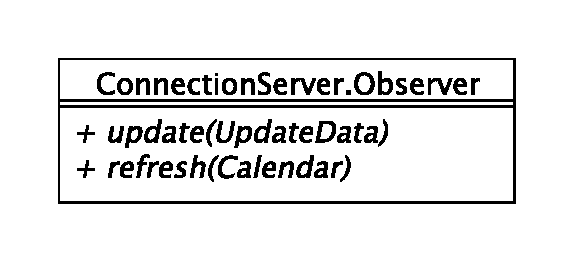
\includegraphics[scale=0.7]{diagrams/vms-class-diagram.eps}
\end{figure}
These are the classes involved to update the data for the graphical interface. The RadarGUI class is where the user can see the output and is updated by a notification from RadarMonitor.
The RadarMonitor keeps track of the state of vessels within its range. It issues alerts to its observers whenever they occur. It receives UpdateData from clients via notifications from the ConnectionServer class.

The ConnectionServer class abstracts away the implementation details of receiving an UpdateData from a client over the network; it does not care whether the client is a Simulator program, or a real vessel (both use the same network protocol and data format).

\break
\begin{figure}[!htb]
\caption{Communication Diagram of the Vessel Monitoring System (VMS) Subsystem}
\centering
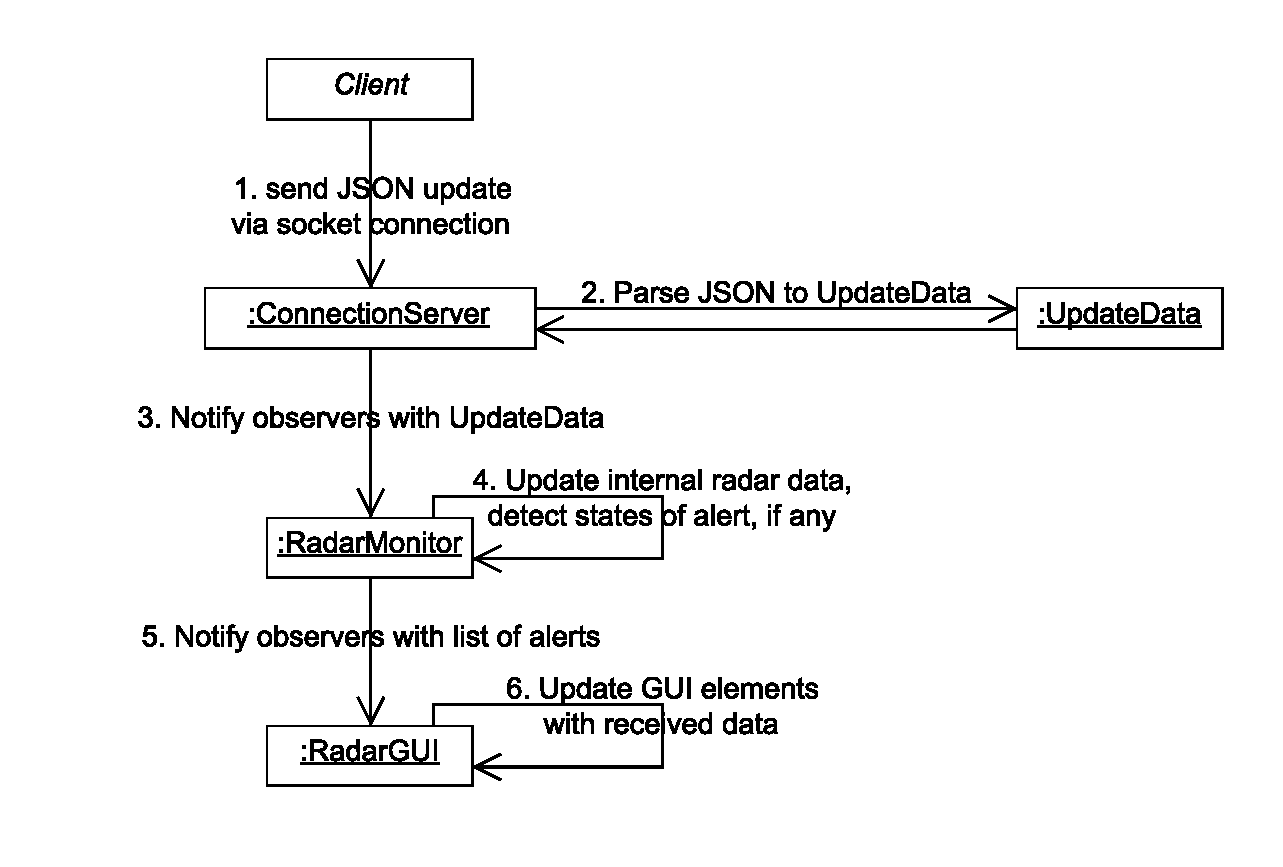
\includegraphics[scale=0.7]{diagrams/vms-communication-diagram.eps}
\end{figure}
When the program is started, the ConnectionServer instance will bind to a specific address and listen for JSON updates from any connected clients. When an UpdateData is received and parsed successfully, it will notify its observers that the data has been changed. The main observer of ConnectionServer is the RadarMonitor instance. Inside the radar monitor it will search for any data that requires attention (e.g. alerts). If any need attention, it will notify the observers (RadarGUI) with the list of alerts, and they will be displayed to the user.

\break
\subsubsection{Process View} % Status: Complete

\begin{figure}[!htb]
\caption{Activity Diagram for the Simulator Subsystem}
\centering
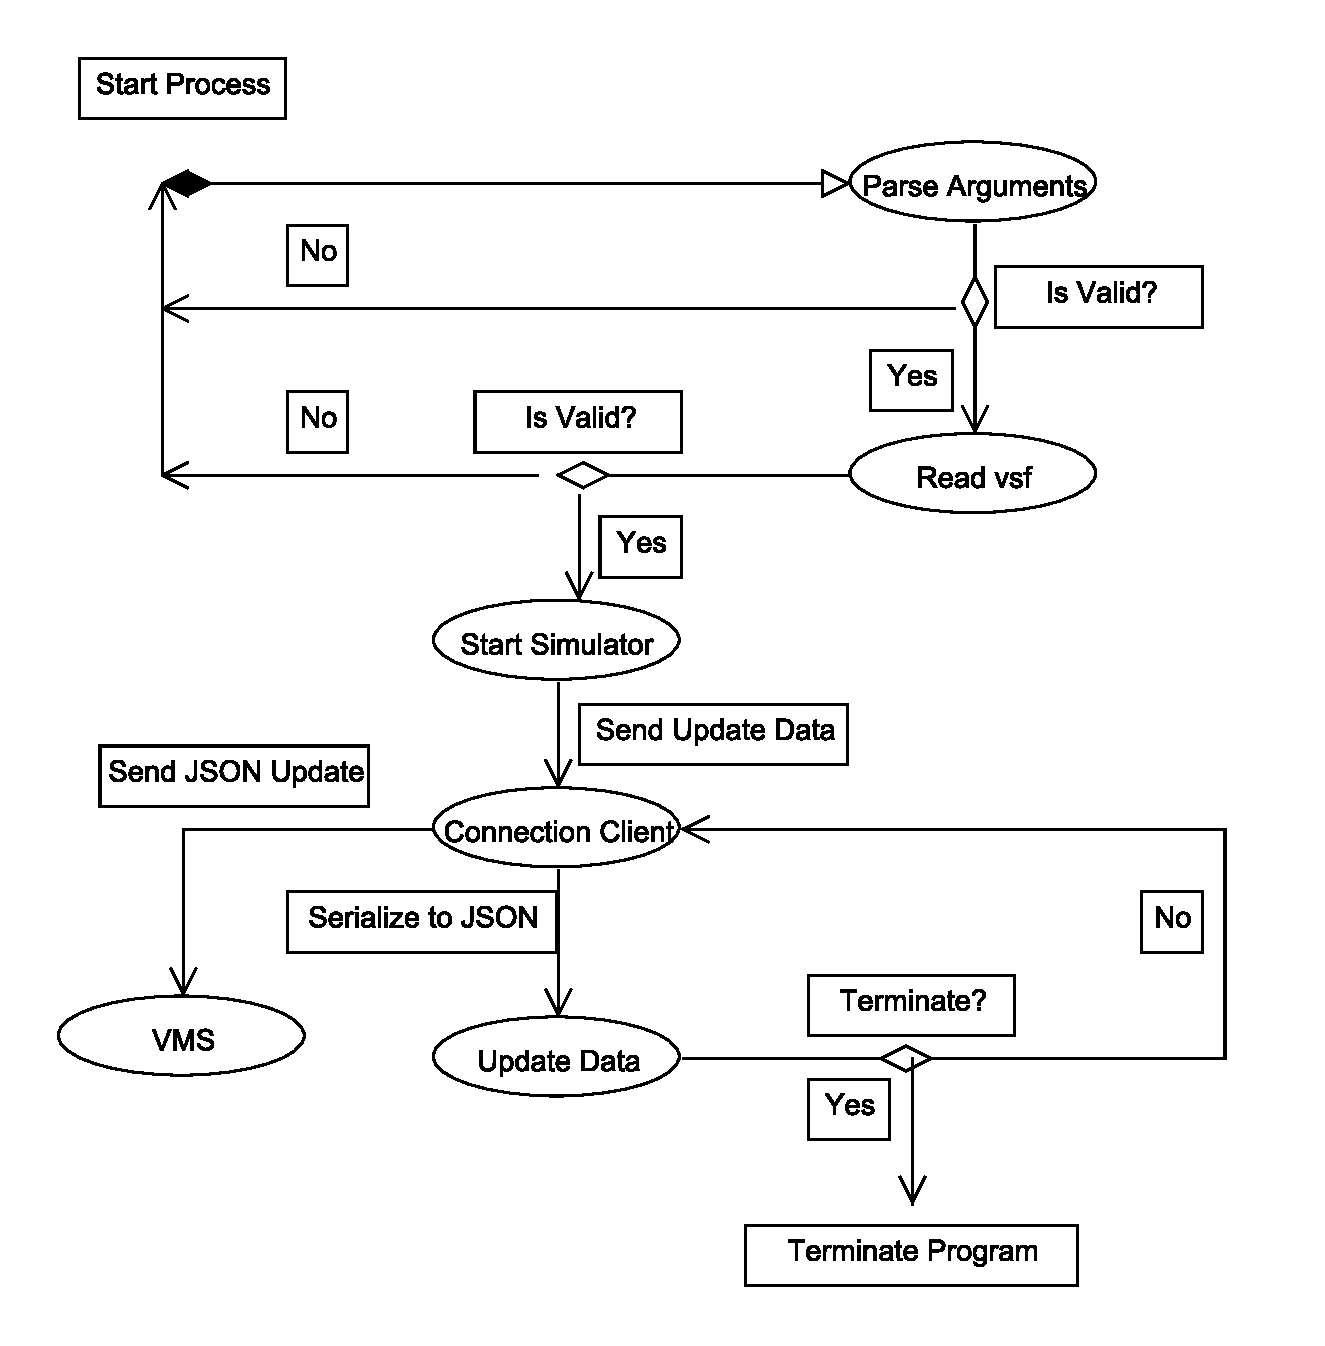
\includegraphics[scale=0.7]{diagrams/simulator-acitivity-diagram.eps}
\end{figure}
The simulator has two main functionality: validating input from user and initializing/updating the data. The first step is to validate the parameters given from the user, it will check if the host, port and the .vsf file. If anything fails in step one the program will exit and wait for the user to input the next command line. Then step two happens, it will start the simulator, use the data received, and send it to the connection client. Connection client will serialize the data to update data and will keep looping around till the program terminates.

\break
\begin{figure}[!htb]
\caption{Activity Diagram for the Vessel Monitoring System (VMS) }
\centering
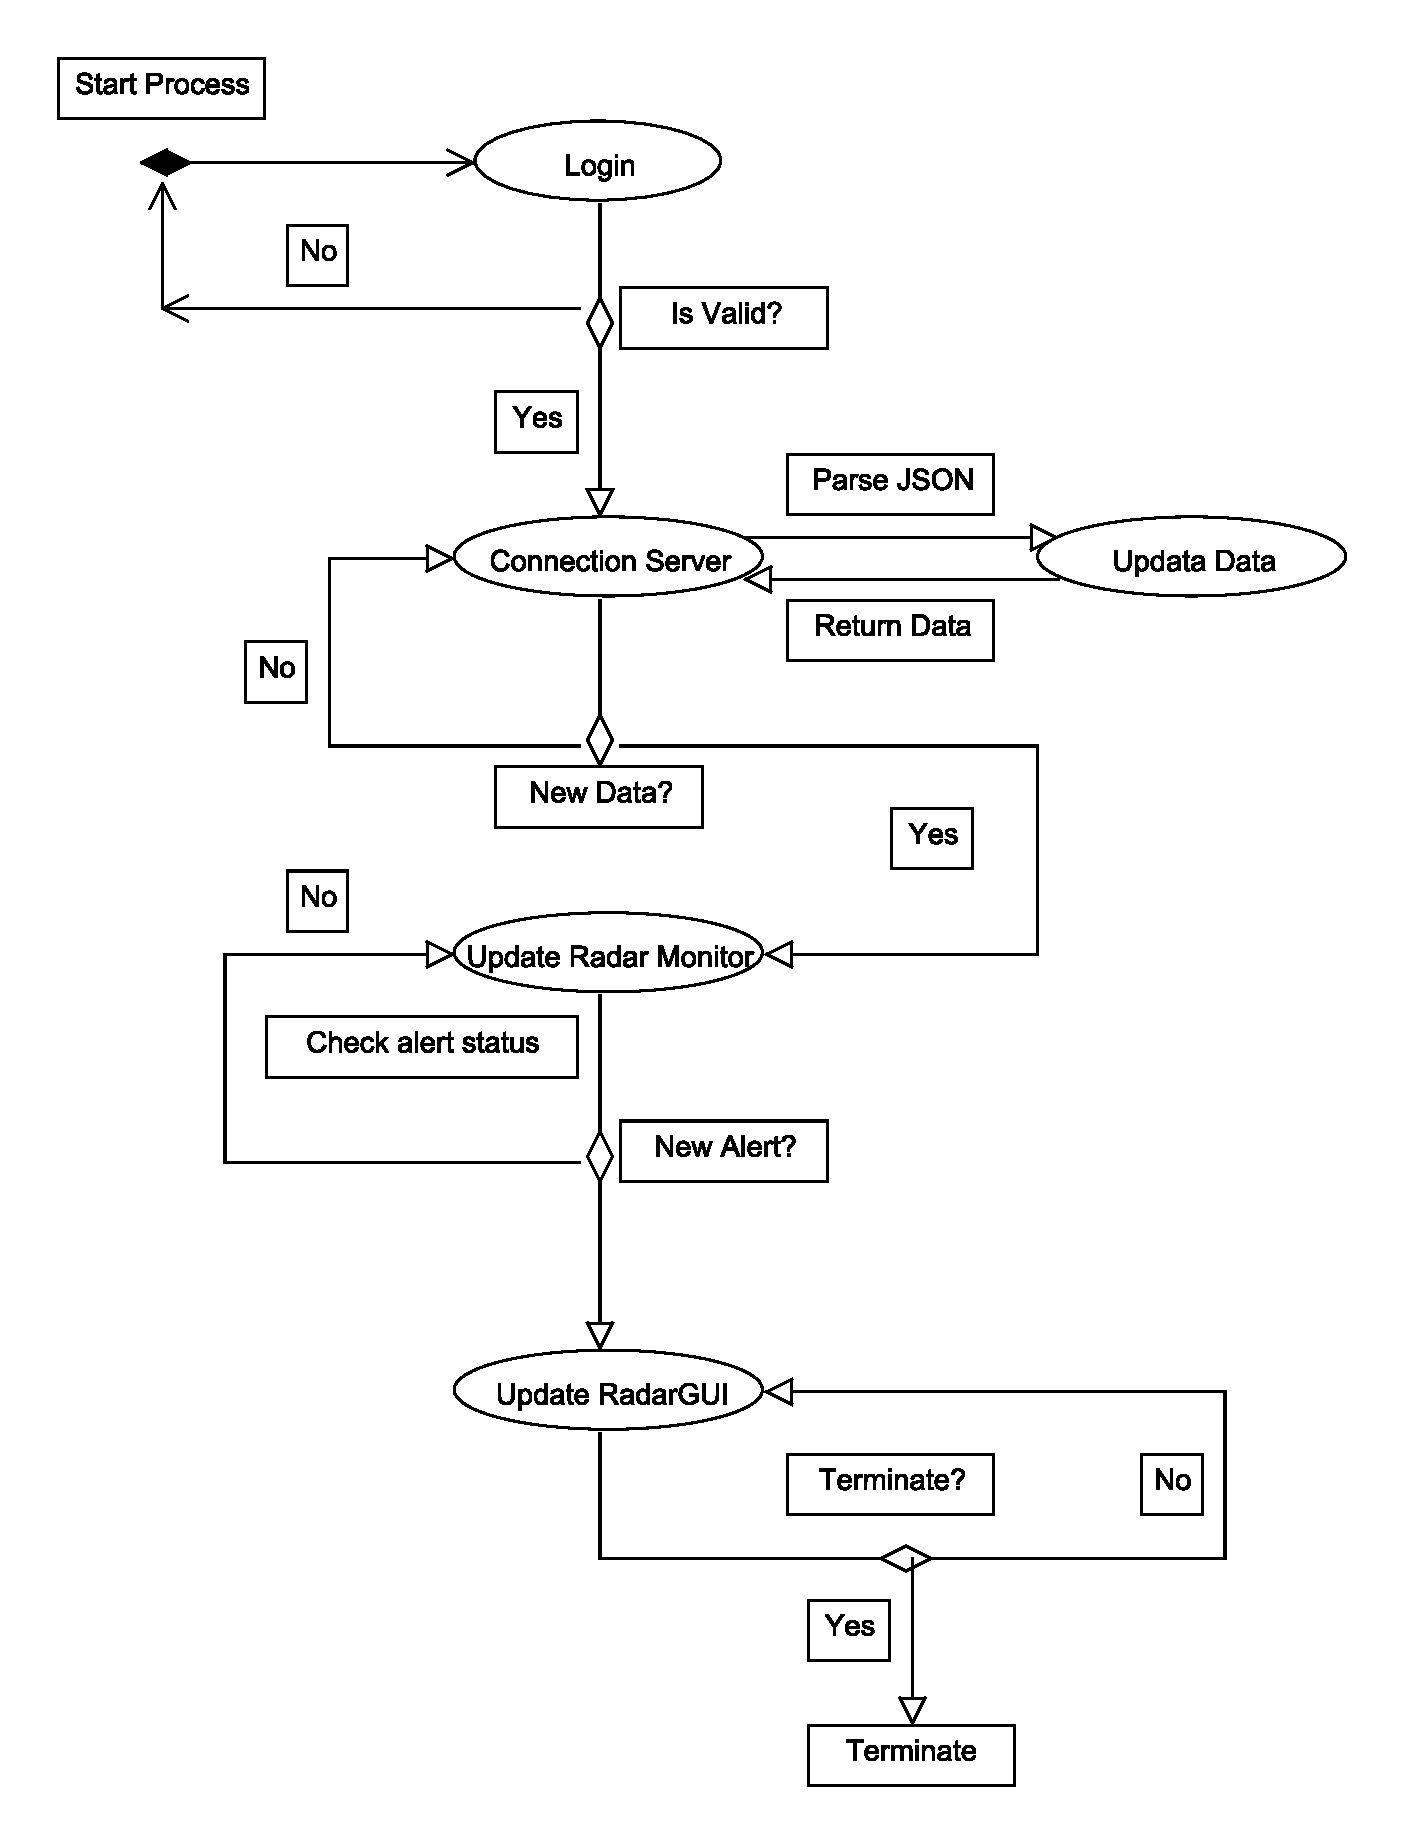
\includegraphics[scale=0.6]{diagrams/vms-activity-diagram.eps}
\end{figure}
The Vessel Monitoring System has two main functionality: connecting to server and updating the graphical user interface with the data. The first step is to connect to then server, in this step the user will be connected via socket to the server. If it fails it will simply return to the start. Then step two happens, the connection server will request data from update data. If new data was found it will send it to the radar monitor. Then when the radar monitor receives the new data it will check if any alert were triggered and update the graphical user interface.

\break
\subsubsection{Development View} % Status: Complete
\begin{figure}[!htb]
\caption{Component Diagram of the Vessel Monitoring System (VMS)}
\centering
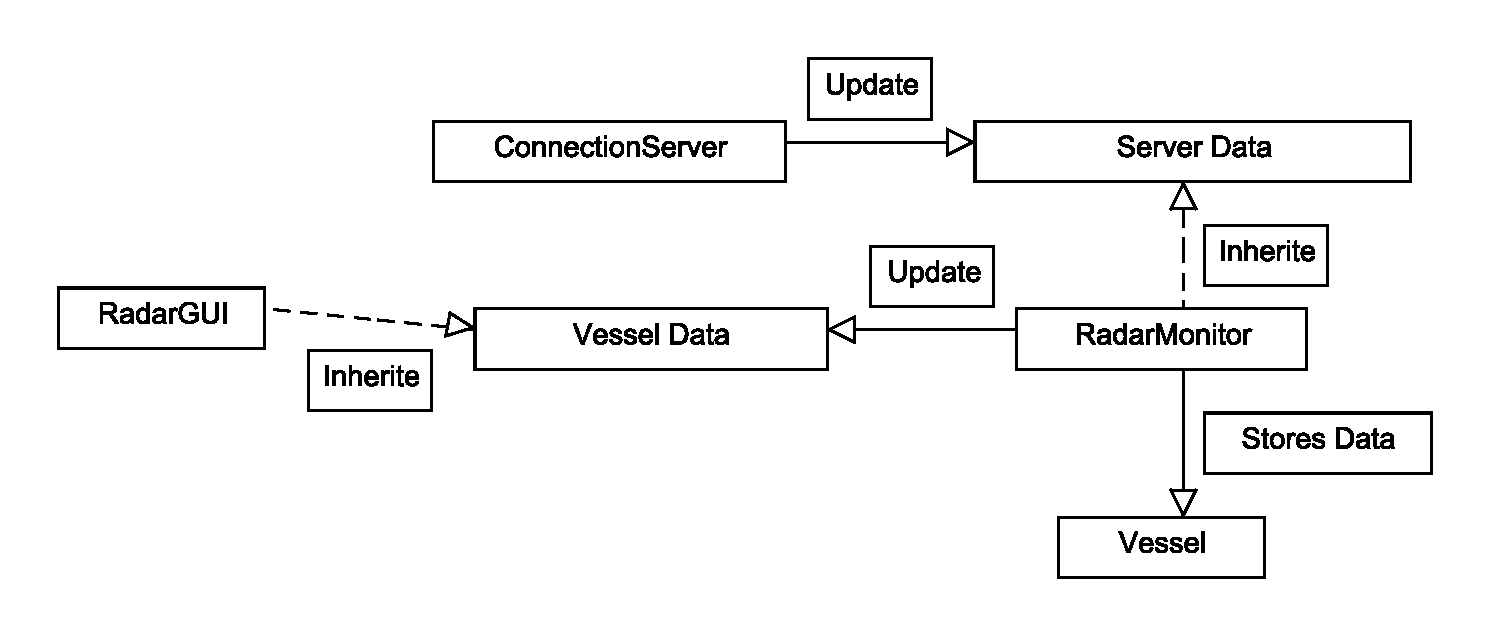
\includegraphics[scale=0.7]{diagrams/vms-component-diagram.eps}
\end{figure}
In the Vessel Monitoring System, the RadarMonitor is the core of this subsystem. The information of the server is recorded in RadarMonitor. It also updates the information that is sent to the user interface.

\begin{figure}[!htb]
\caption{Component Diagram of the Simulator}
\centering
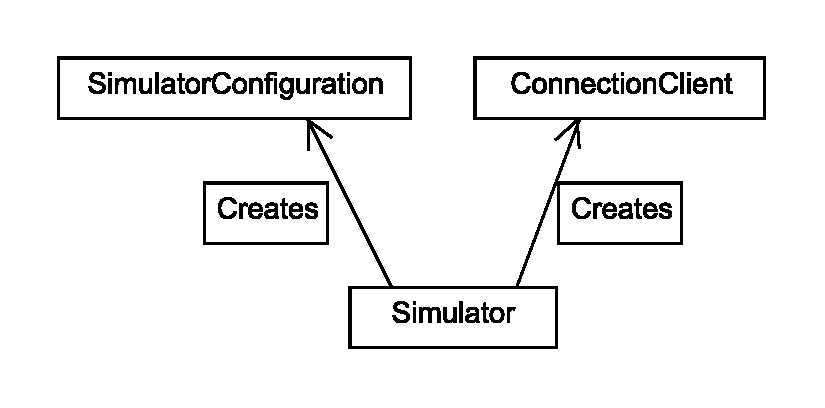
\includegraphics[scale=0.7]{diagrams/simulator-component-diagram.eps}
\end{figure}
In the Simulator subsystem, the simulator itself is the core.
From the simulator, it goes ahead and create an instance of SimulatorConfiguration and ConnectionClient.
With those in hand, it will be able to start the simulation.

\break
\subsubsection{Scenarios} % Status: Complete

\begin{figure}[!htb]
\caption{Use Case Diagram for the Simulator}
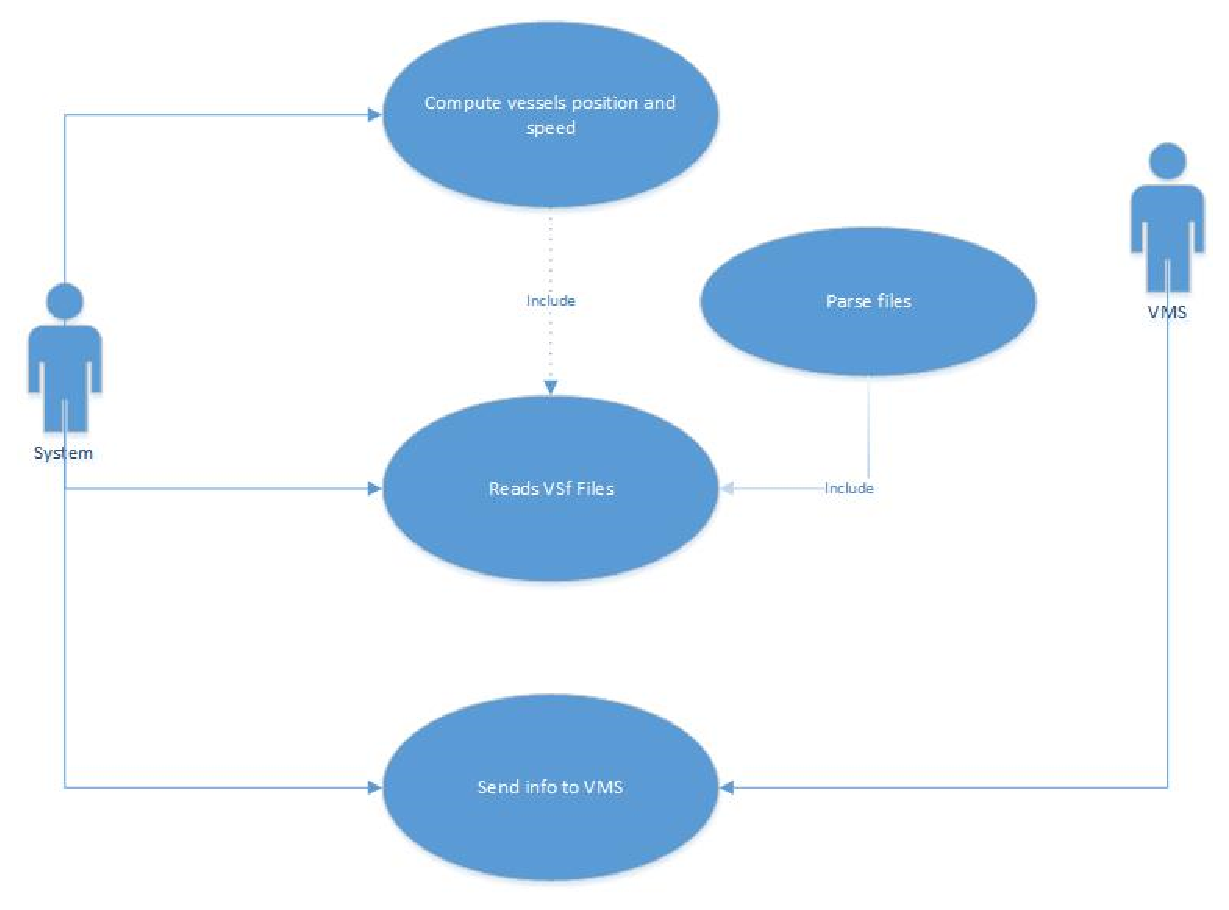
\includegraphics[scale=0.4]{diagrams/usecasediagram.eps}
\end{figure}
The Simulator in general when started, the system will parse the settings and read the .vsf file. From there it will send it to the server where the Vessel Monitoring System can retrieve it.

\break

\begin{figure}[!htb]
\caption{Use Case Diagram for the Vessel Monitoring System (VMS)}
\centering
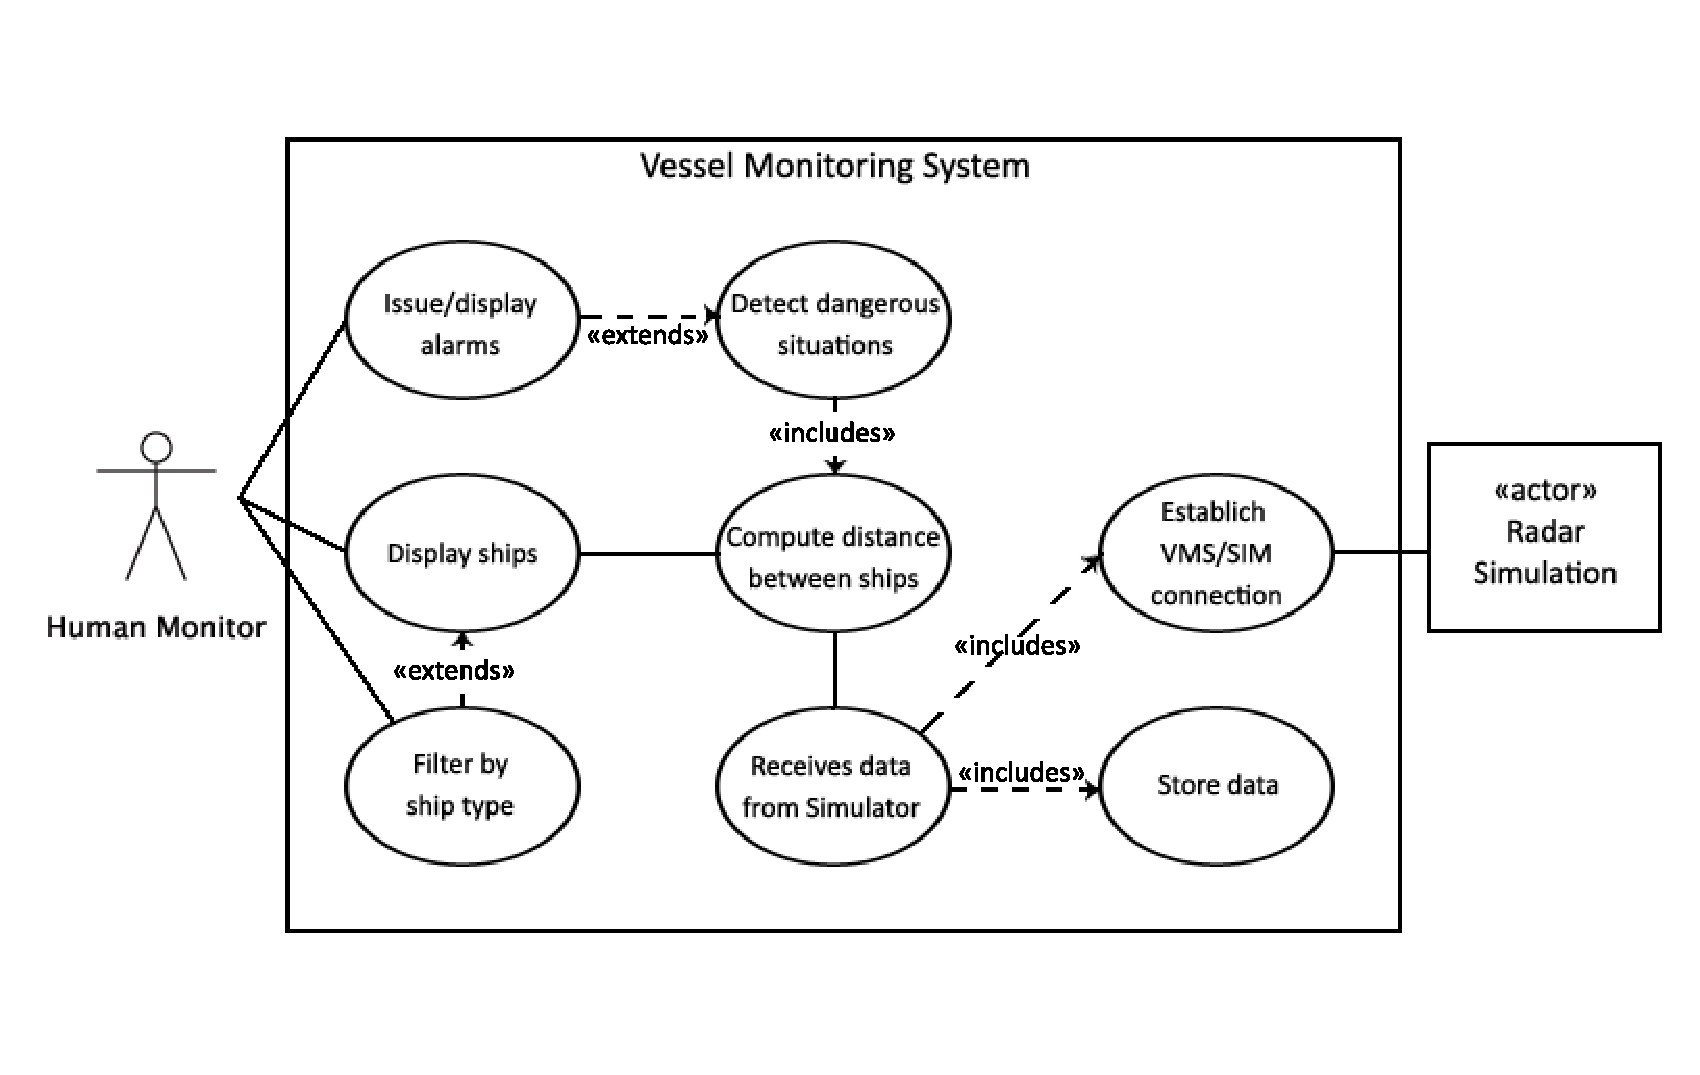
\includegraphics[scale=0.32]{diagrams/vmsdiagram.eps}
\end{figure}
The Vessel Monitoring System system is where the user can interact with the data. He can either look at the data or a subset of the data. 
The information is supplied by the Radar Simulator and sent to the VMS.
Then with that data the VMS checks if any alerts are needed to be outputed to the user.

\subsection{Subsystem Interfaces Specifications} % Status: See subsubsections

\subsubsection{Simulator subsystem} % Status: Complete

\begin{enumerate}
  \item Parse command-line invocation from user: 
		\begin{verbatim}
		"./Simulator --host 192.168.0.1 --port 1024 --input filename.vsf"
		\end{verbatim}
		Note: \verb|--host|, \verb|--port| and \verb|--input| can be replaced with \verb|-h|, \verb|-p|, \verb|-i| respectively.
		\newline The arguments must be entered in this order.
  \item In the main method, it will be ensured that the command-line invocation is written as it is above, otherwise the program will exit.
  \item When all cleared, \verb|"SimulatorConfiguration.parseVSF(InputStream in)"| will return the configuration instance of the simulator.
  \item Any files that are opened at this time will be closed to ensure no unnecessary streams are open.
	\item \verb|"ConnectionClient.connect(String host, int port)|" will take the validated host and port from the command-line and create a new socket for the user.
	\item \verb|"Simulator.start(ConnectionClient client)"| will take the client instance created in step 5 and use it to start the simulator.	
\end{enumerate}

\subsubsection{VMS subsystem} % Status: Complete

\begin{enumerate}
	\item	Create a ConnectionServer instance
	\item Create a RadarMonitor instance
	\item Register RadarMonitor as an observer of ConnectionServer using:
		\newline \verb|"ConnectionServer.registerObserver(Observer o)"|
	\item Run \verb|"ConnectionServer.start()"|
	\item  Create vms.gui.Login instance, show the window
	\item After user has logged in, create vms.gui.RadarDisplay instance
	\item Register RadarDisplay instance as observer of RadarMonitor
	\item Show RadarDisplay window
\end{enumerate}

\break

\section{Detailed Design} % Status: Complete

In this section, we will describe in detail each subsystem of the software.

\subsection{Subsystems} % Status: Complete

\subsubsection{Detailed Design Diagram} % Status: Complete

\paragraph{Simulator Subsystem} 

\begin{figure}[!htb]
\caption{Simulator Class Diagram}
\centering
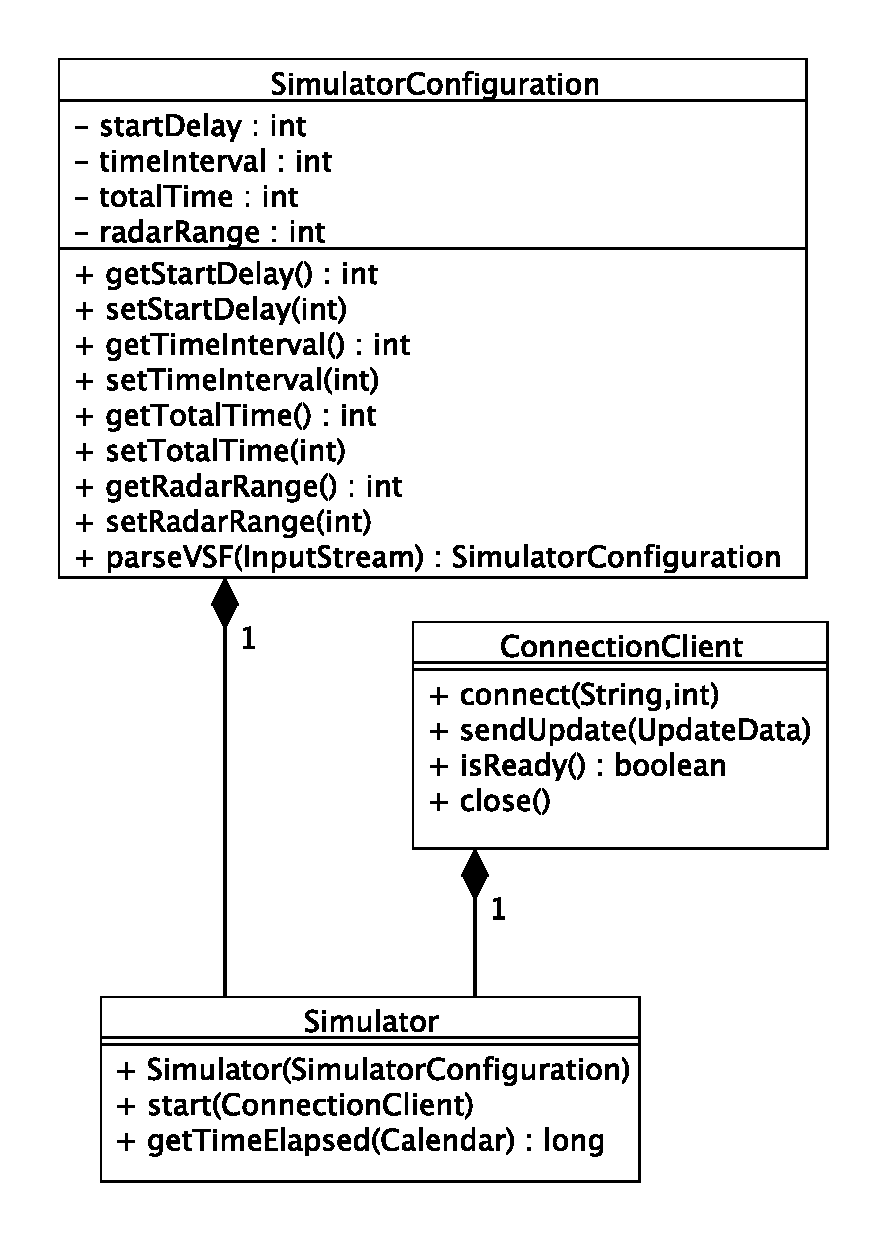
\includegraphics[scale=0.7]{diagrams/simulator-class-diagram.eps}
\end{figure}
The Simulator subsystem is the part of the software that will simulate the actual physical radar and the data it sends to the Vessel Monitoring System (VMS). A .vsf file, which lists the positions and courses of given vessels, as well as various configuration parameters for the VMS, is parsed and interpreted as vessel data by the simulator, which then establishes socket communication with the VMS. The simulator then proceeds to send updated data to the VMS at set intervals, until the pre-defined total time limit expires.

\break
\paragraph{Vessel Monitoring System (VMS) Subsystem}

\begin{figure}[!htb]
\caption{VMS Class Diagram}
\centering
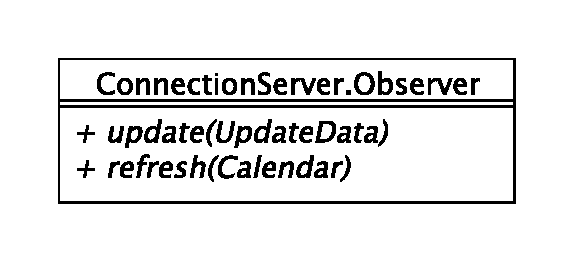
\includegraphics[scale=0.7]{diagrams/vms-class-diagram.eps}
\end{figure}
The Vessel Monitoring System (VMS) subsystem is the part of the software that will receive vessel data from the radar (represented by the Simulator) and interpret this data so that it can be viewed by the user via a graphical interface, and emit high- or low-risk alerts if any two vessels are within a certain range of each other. The VMS accepts socket connections from any number of Simulator instances.

\break
\subsubsection{Unit Descriptions} % Status: Complete

\paragraph{Simulator Subsystem}

\subparagraph{Class SimulatorConfiguration}
The main purpose of this class is to parse the .vsf file and to keep track of the data obtained, as well as registering any modifications to this data.

\vspace{0.5cm}
Attributes:
\begin{enumerate}
    \item private int \_StartDelay
    \item private int \_TimeInterval
    \item private int \_TotalTime
    \item private int \_RadarRange
    \item List\textless Vessel\textgreater \, \_Vessels
\end {enumerate}

\vspace{0.5cm}
Functions:
\begin{enumerate}
	\item private SimulatorConfiguration()
	\item public int getStartDelay()
	\item public void setStartDelay(int)
	\item public int getTimeInterval()
	\item public void setTimeInterval(int)
	\item public int getTotalTime()
	\item public void setTotalTime(int)
	\item public int getRadarRange()
	\item public void setRadarRange(int)
	\item public List\textless Vessel\textgreater  \,getVessels()
	\item public void addVessel(Vessel)
	\item public static SimulatorConfiguration parseVSF(InputStream)
\end{enumerate}

\break
\subparagraph{Class ConnectionClient}
This class is responsible for establishing and managing the socket connection to the VMS, as well as sending all update data via this connection. The sent data is converted to JSON and encoded as Netstring.

\vspace{0.5cm}
Attributes:
\begin{enumerate}
	\item private final int TIMEOUT
    \item private Socket \_Socket
\end {enumerate}

\vspace{0.5cm}
Functions:
\begin{enumerate}
	\item public ConnectionClient()
	\item public void connect(String, int)
	\item public void sendUpdate(UpdateData)
	\item public boolean isReady()
	\item public void close()
\end{enumerate}

\subparagraph{Class Simulator}
This class performs and determines the frequency of data updates and communications to the VMS. Once a connection to the VMS is established, the Simulator creates a thread for a set duration, during which the data from SimulatorConfiguration is updated and sent to VMS through the ConnectionClient at set intervals.

\vspace{0.5cm}
Attributes:
\begin{enumerate}
	\item SimulatorConfiguration \_Configuration
\end {enumerate}

\vspace{0.5cm}
Functions:
\begin{enumerate}
	\item public Simulator(SimulatorConfiguration)
	\item public void start(ConnectionClient)
	\item public long getTimeElapsed(Calendar)
\end{enumerate}

\paragraph{Vessel Monitoring System (VMS) Subsystem}

\subparagraph{Class ConnectionServer}
The purpose of this class is to accept connections established by one or more radars, and receive the transmitted data. In addition, observers may be registered so that they will be notified of every incoming data update.

\vspace{0.5cm}
Attributes:
\begin{enumerate}
	\item private static long DEFAULT\_REFRESH
    \item private boolean \_Continue
    \item private long \_RefreshTime
    \item private Selector \_Selector
    \item private ServerSocketChannel \_Channel
    \item private List\textless Observer\textgreater \,\_Observers
\end {enumerate}

\vspace{0.5cm}
Functions:
\begin{enumerate}
	\item public ConnectionServer()
	\item public void setMinimumRefresh(long)
	\item public long getMinimumRefresh()
	\item public void registerObserver(Observer)
	\item public void unregisterObserver(Observer)
	\item public void refreshObservers(Calendar)
	\item public void updateObservers(UpdateData)
	\item public void bind(SocketAddress)
	\item public void setRadarRange(int)
	\item public List\textless Vessel\textgreater \,getVessels()
	\item public void addVessel(Vessel)
	\item public static SimulatorConfiguration parseVSF(InputStream)
\end{enumerate}

\subparagraph{Class RadarMonitor (implements ConnectionServer.Observer)}
This class stores and updates any vessel data received by the ConnectionServer.

\vspace{0.5cm}
Attributes:
\begin{enumerate}
	\item private Coord lowerRange
    \item private Coord upperRange
    \item private ArrayList\textless Vessel\textgreater \,\_Vessels
    \item private List\textless Observer\textgreater \,\_Observers
\end {enumerate}

\vspace{0.5cm}
Functions:
\begin{enumerate}
	\item public void setRange(Coord, Coord)
	\item public int getVesselCount()
	\item public List\textless Vessel\textgreater \,getVessels()
	\item public void registerObserver(Observer)
	\item public void unregisterObserver(Observer)
	\item public void update(UpdateData)
	\item public void refresh(Calendar)
\end{enumerate}

\break
\subparagraph{Class RadarDisplay (implements RadarMonitor.Observer)}
This class displays the data maintained by the RadarMonitor, using GUI components.

\vspace{0.5cm}
Attributes: (none)

\vspace{0.5cm}
Functions:
\begin{enumerate}
	\item public RadarDisplay()
	\item public void refresh(List\textless Alert\textgreater \,)
\end{enumerate}

\subparagraph{Class Vessel}
This class represents a vessel and all of its relevant characteristics.

\vspace{0.5cm}
Attributes:
\begin{enumerate}
	\item private VesselType type
    \item private String id
    \item private Course course
    \item private Coord coords
    \item private Calendar lastTimestamp
\end {enumerate}

\vspace{0.5cm}
Functions:
\begin{enumerate}
	\item public Vessel(String, VesselType)
	\item public String getId()
	\item public VesselType getType()
	\item public Coord getCoord(Calendar)
	\item public Course getCourse(Calendar)
	\item public Calendar getLastTimestamp()
	\item public void update(Coord, Course, Calendar)
	\item public void update(UpdateData)
	\item public UpdateData getUpdateData(Calendar)
\end{enumerate}

\section{Dynamic Design Scenarios} % Status: Complete

In this section, we introduce two possible scenarios (use cases), which show interactions between the software and external users. In addition, we show how components of the software interact, within each subsystem.

\break
\subsection{Use Case Scenarios}

Here, we present the interactions between the software and external users.

\paragraph{Scenario 1: User}

\begin{figure}[!htb]
\caption{Sequence Diagram - User}
\centering
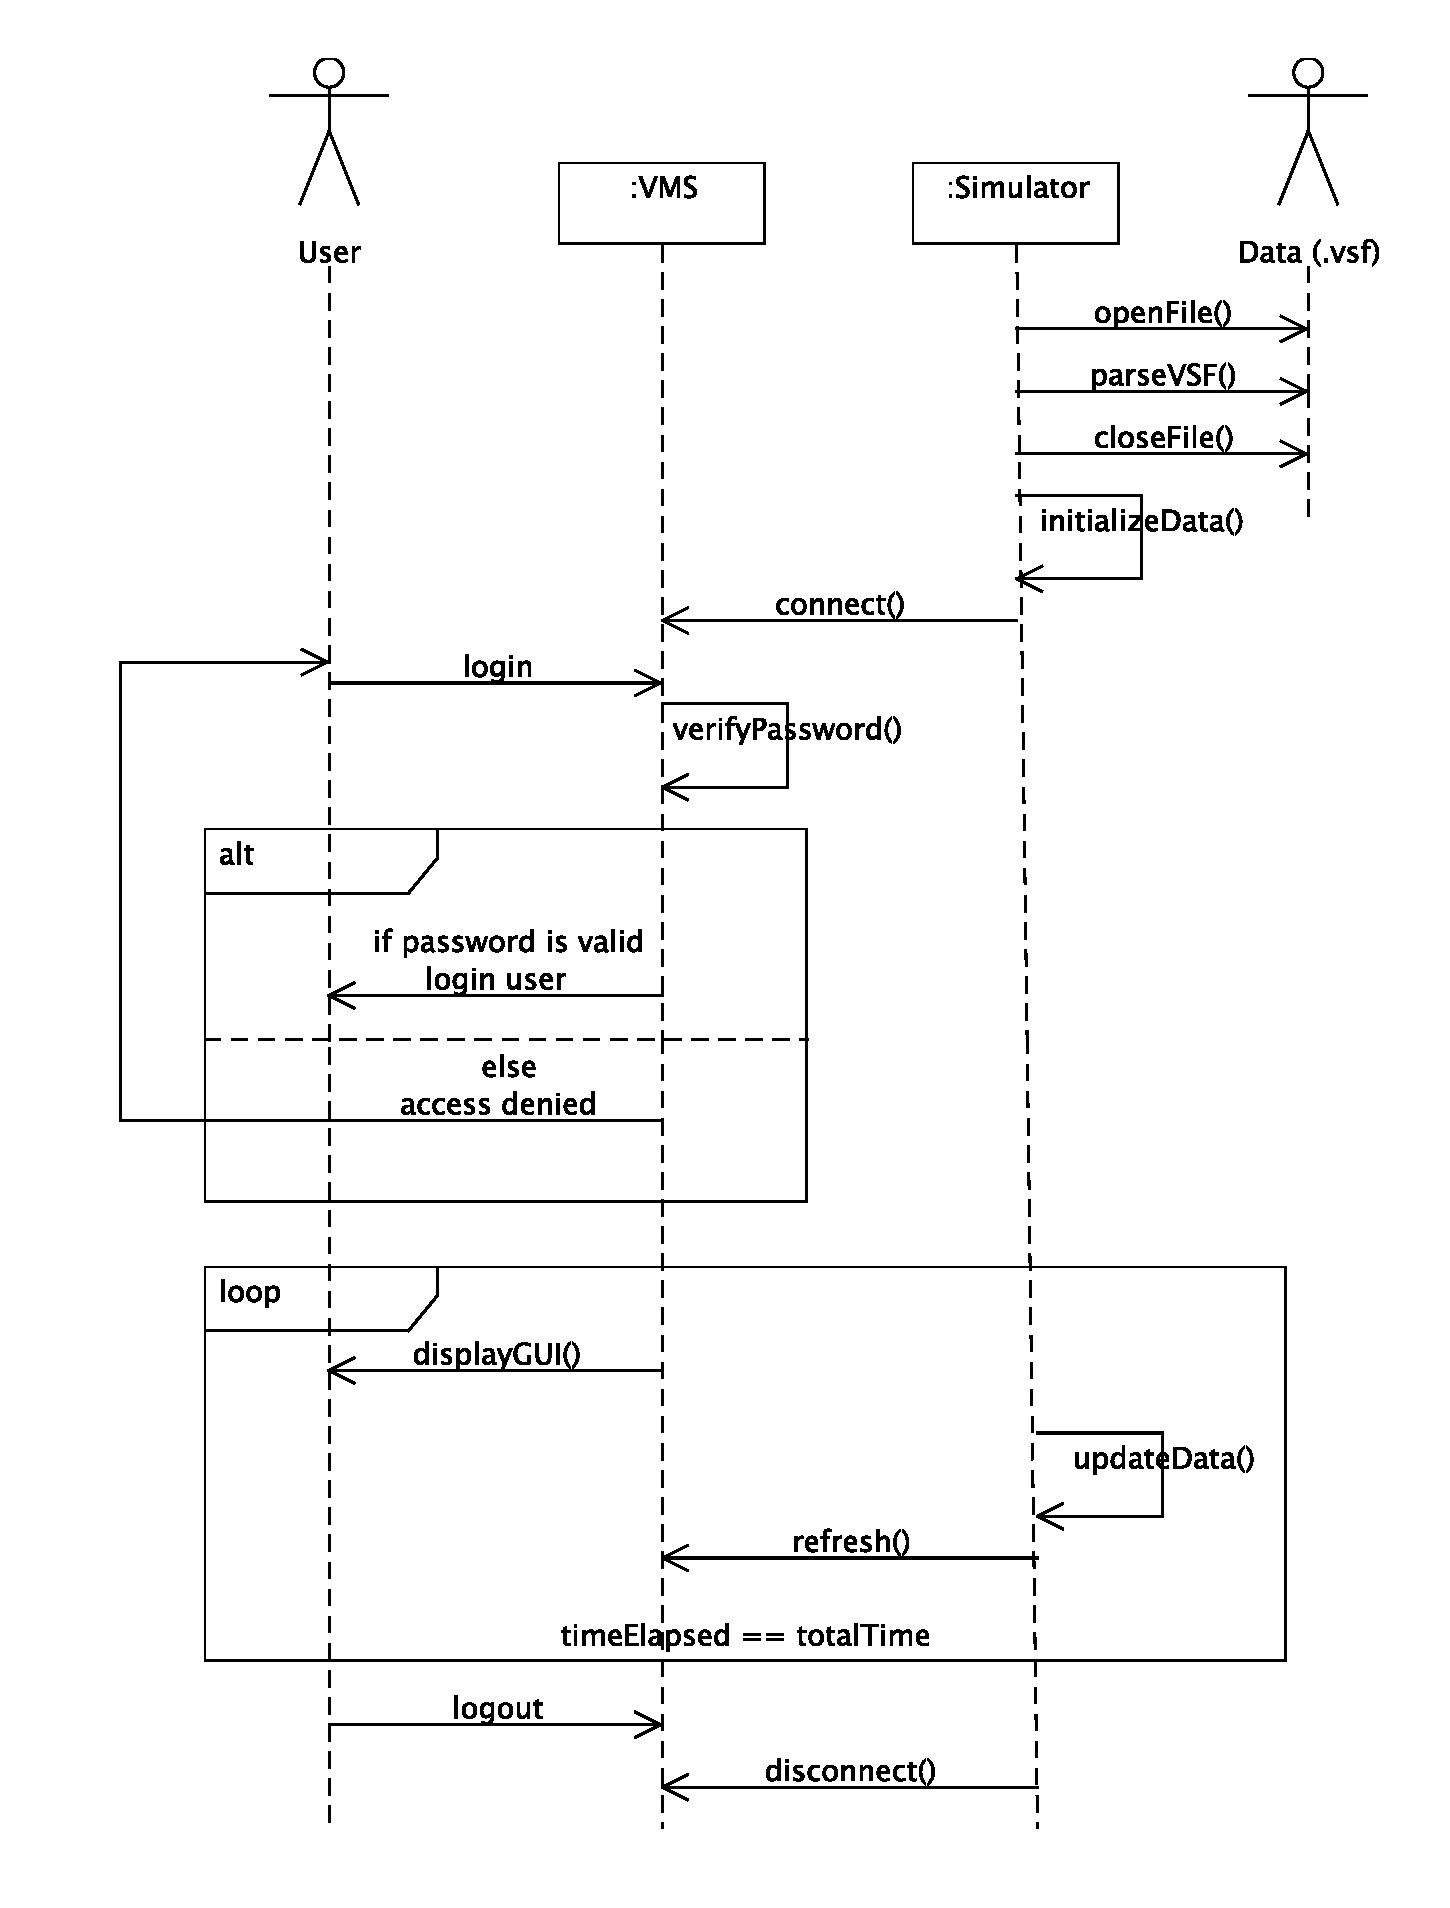
\includegraphics[scale=0.6]{diagrams/user-sequence-diagram.eps}
\end{figure}

This scenario represents the interactions between the software and a user with normal access rights ("User").

\subparagraph{Operational Contracts for Scenario 1:}

\begin{description}
  \item[Operation: openFile()] Pre-conditions: valid file name and path were provided.\newline
  Post-conditions: stream to .vsf file is created.
  \item[Operation: parseVSF()] Pre-conditions: .vsf file was correctly opened, and stream was created.\newline
  Post-conditions: text from .vsf file is read by the system.
  \item[Operation: closeFile()] Pre-conditions: .vsf file was opened.\newline
  Post-conditions: none.
  \item[Operation: initializeData()] Pre-conditions: all data parsed from .vsf file were of correct value type and range.\newline
  Post-conditions: text from .vsf file is converted to vessel and configuration data.
  \item[Operation: verifyPassword()] Pre-conditions: user has entered a password.\newline
  Post-conditions:\newline
  - If password is recognized as valid: GUI display is created.\newline
  - If password is not recognized as valid: none.
  \item[Operation: displayGUI()] Pre-conditions: none.\newline
  Post-conditions: any vessel data from the system is sent to GUI for display.
  \item[Operation: updateData()] Pre-conditions: none.\newline
  Post-conditions: system vessel data is modified based on calculated time factor.
  \item[Operation: refresh()] Pre-conditions: none.\newline
  Post-conditions: GUI-displayed vessel data corresponds to system vessel data.
\end{description}

\break
\paragraph{Scenario 2: Administrator}

\begin{figure}[!htb]
\caption{Sequence Diagram - Administrator}
\centering
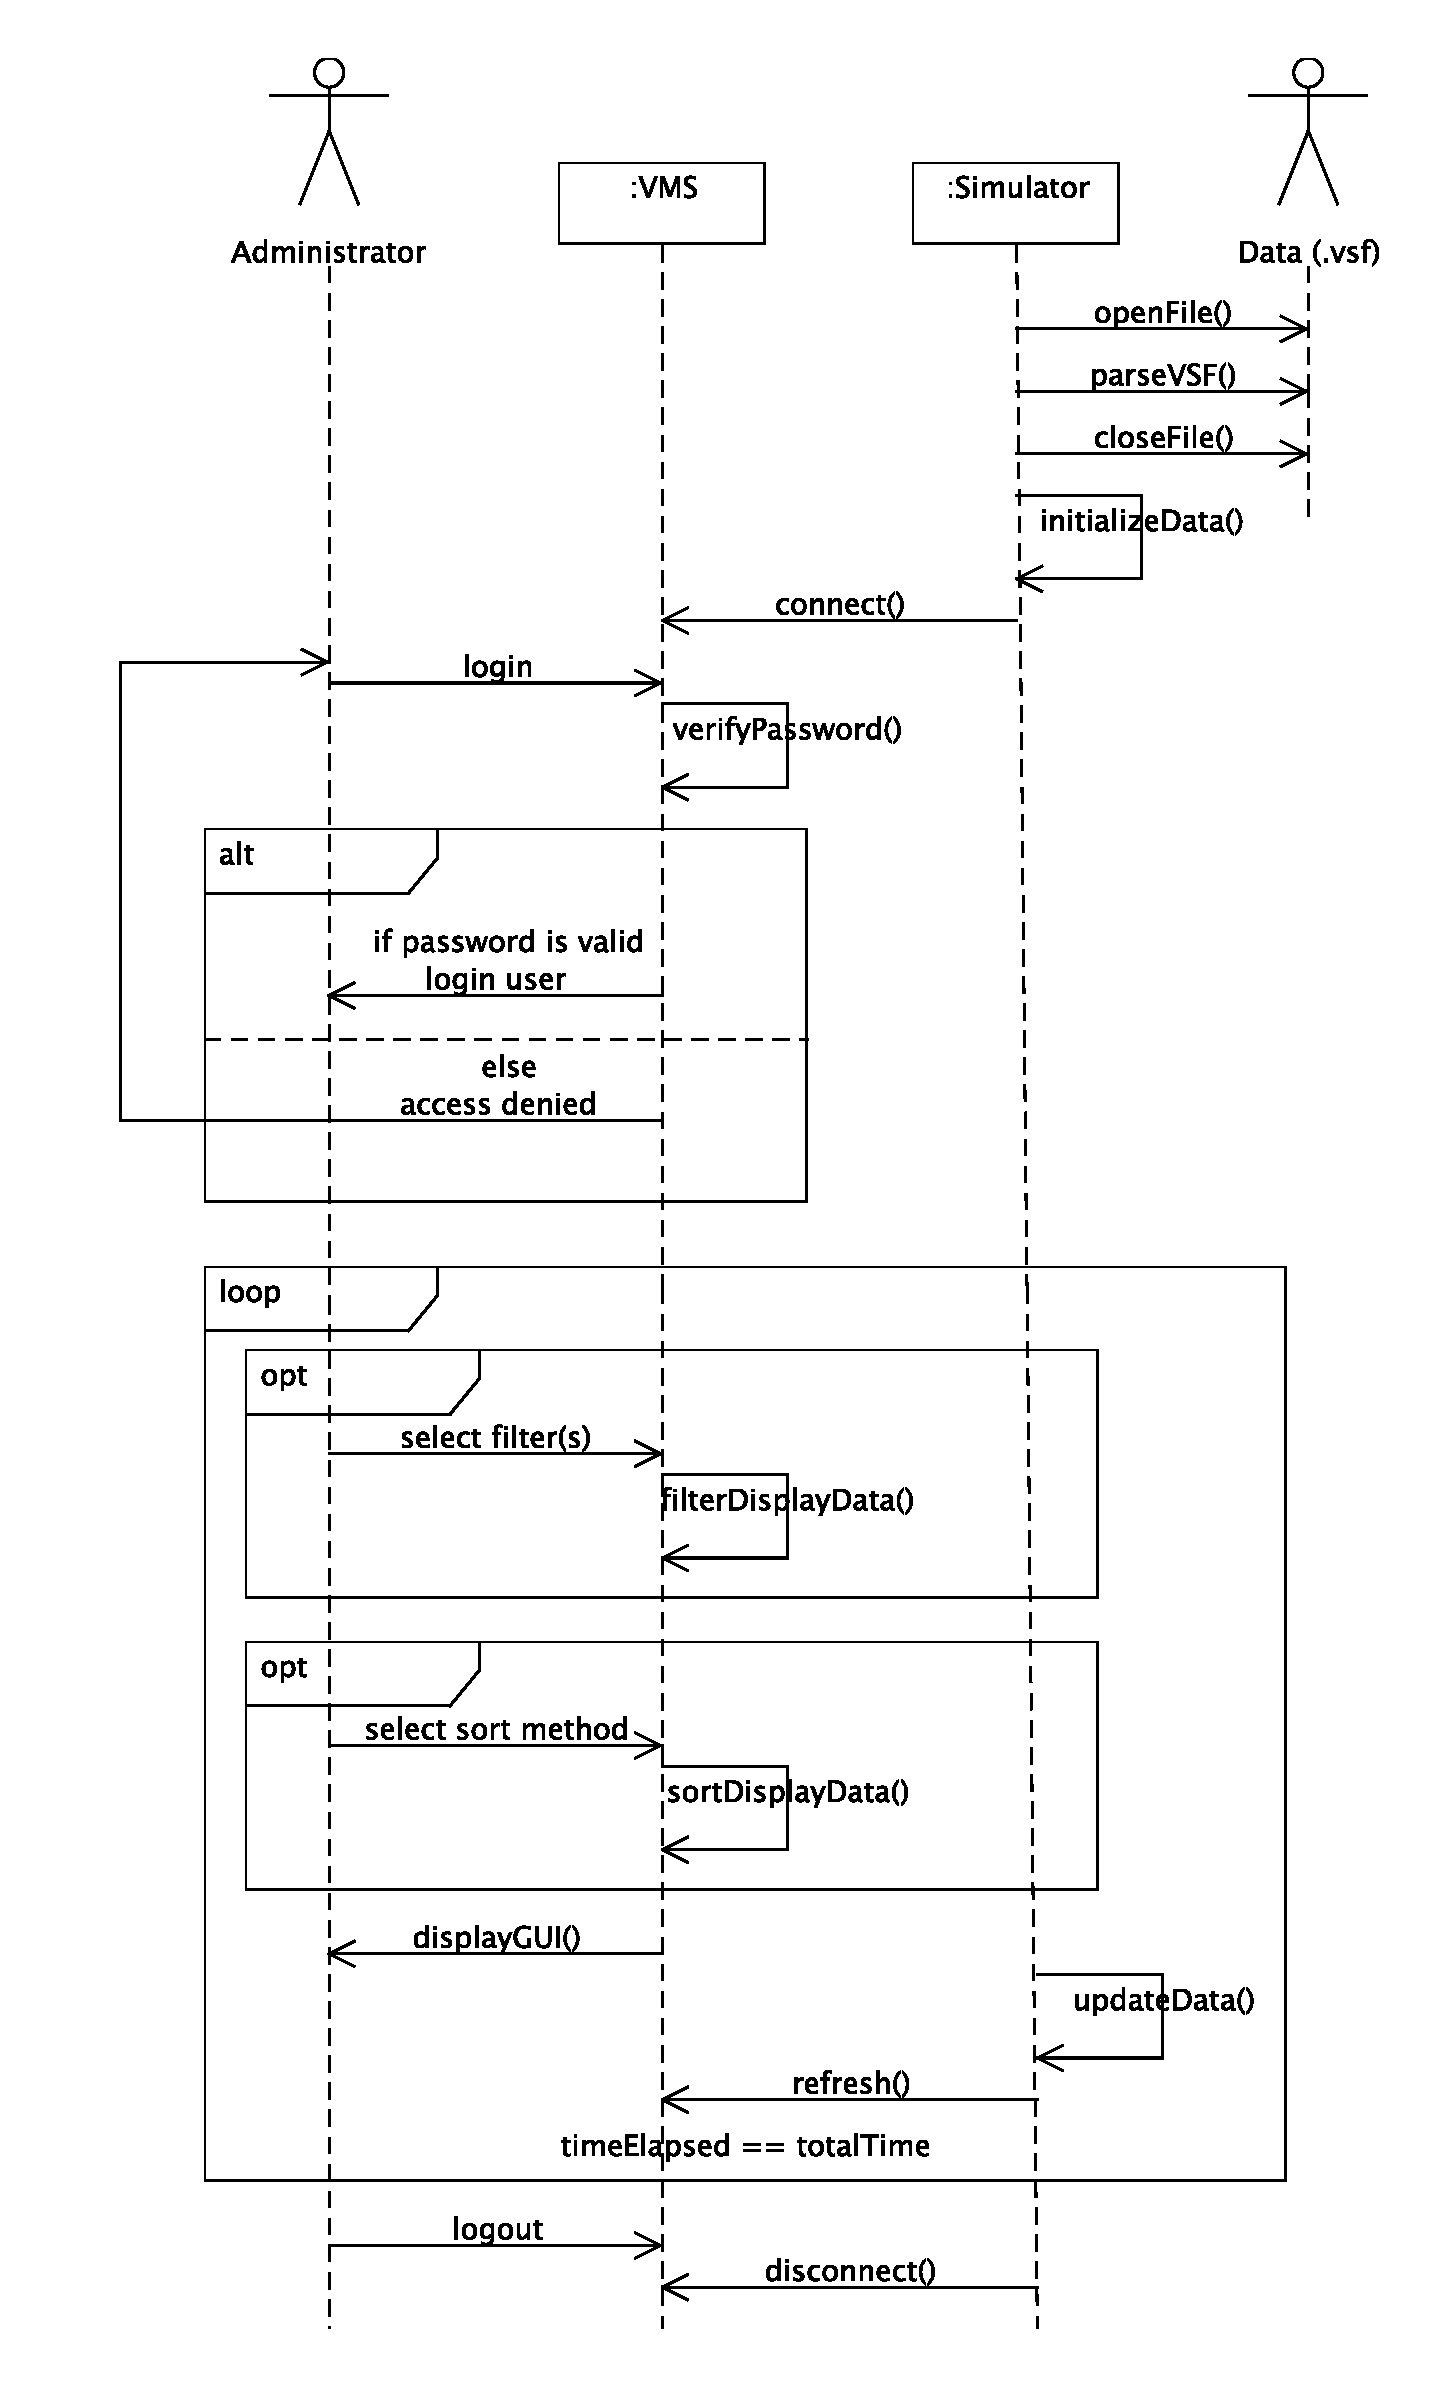
\includegraphics[scale=0.5]{diagrams/admin-sequence-diagram.eps}
\end{figure}

This scenario represents the interactions between the software and a user with full access rights ("Administrator").

\subparagraph{Operational Contracts for Scenario 2:}

Most of the contracts for this scenario are the same as for Scenario 1.

Additional contracts:

\begin{description}
  \item[Operation: filterDisplayData()] Pre-conditions: none.\newline
  Post-conditions: GUI display receives only vessel data allowed by the filter.
  \item[Operation: sortDisplayData()] Pre-conditions: none.\newline
  Post-conditions: GUI displays vessel data based on order specified by the selected sorter.
\end{description}

\subsection{Component Interactions}

Here, we present in more detail the interactions between the system components, which were not shown in the above use case scenarios. We have now abstracted any interactions with external users.

\paragraph{Simulator Subsystem}

\begin{figure}[!htb]
\caption{Sequence Diagram - Simulator}
\centering
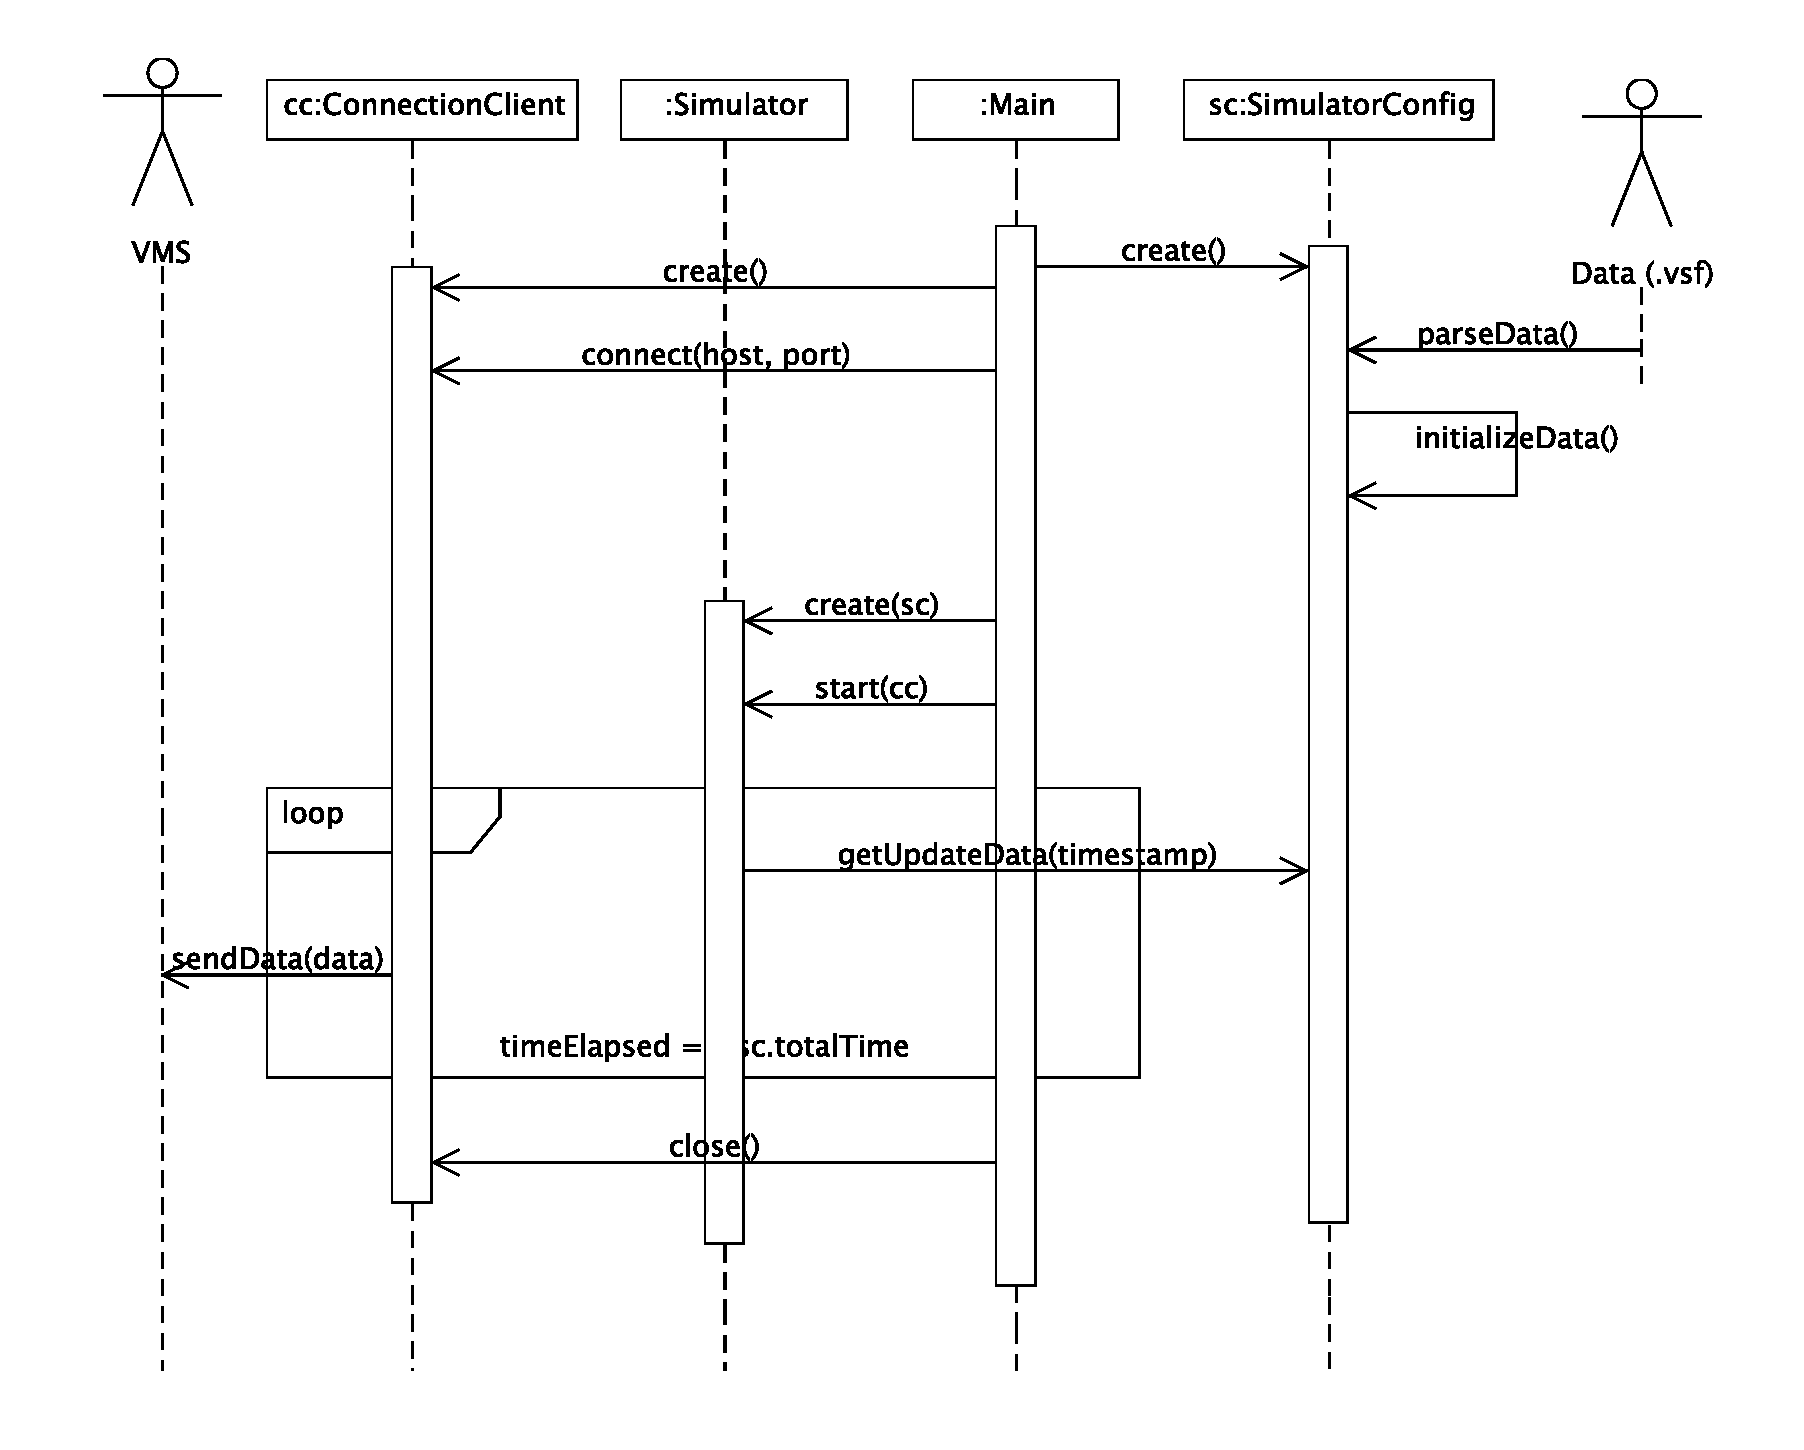
\includegraphics[scale=0.6]{diagrams/simulator-sequence-diagram.eps}
\end{figure}

\subparagraph{Operational Contracts for Simulator Subsystem:}

\begin{description}
  \item[Operation: create() (target: SimulatorConfiguration)] Pre-conditions: none.\newline
  Post-conditions: instance of SimulatorConfiguration is created.
  \item[Operation: create() (target: ConnectionClient)] Pre-conditions: none.\newline
  Post-conditions: instance of ConnectionClient is created.
  \item[Operation: connect(String host, int port)] Pre-conditions: parameter values form a resolvable hostname + port number pair.\newline
  Post-conditions: attempt is made to connect to the server.
  \item[Operation: create(SimulatorConfiguration sc) (target: Simulator)] Pre-conditions: none.\newline
  Post-conditions: instance of Simulator is created.
  \item[Operation: start(ConnectionClient cc)] Pre-conditions: connection to server was established.\newline
  Post-conditions: vessel data is sent to server at set intervals for a given duration, determined by configuration data.
  \item[Operation: getUpdateData(Calendar timestamp)] Pre-conditions: parameter value represents a valid timestamp.\newline
  Post-conditions: updated vessel data is returned.
  \item[Operation: sendUpdate(UpdateData data)] Pre-conditions: none.\newline
  Post-conditions: updated vessel data is sent to server.
  \item[Operation: close()] Pre-conditions: none.\newline
  Post-conditions: Socket is closed.
\end{description}

\break
\paragraph{Vessel Monitoring System (VMS) Subsystem}

\begin{figure}[!htb]
\caption{Sequence Diagram - VMS}
\centering
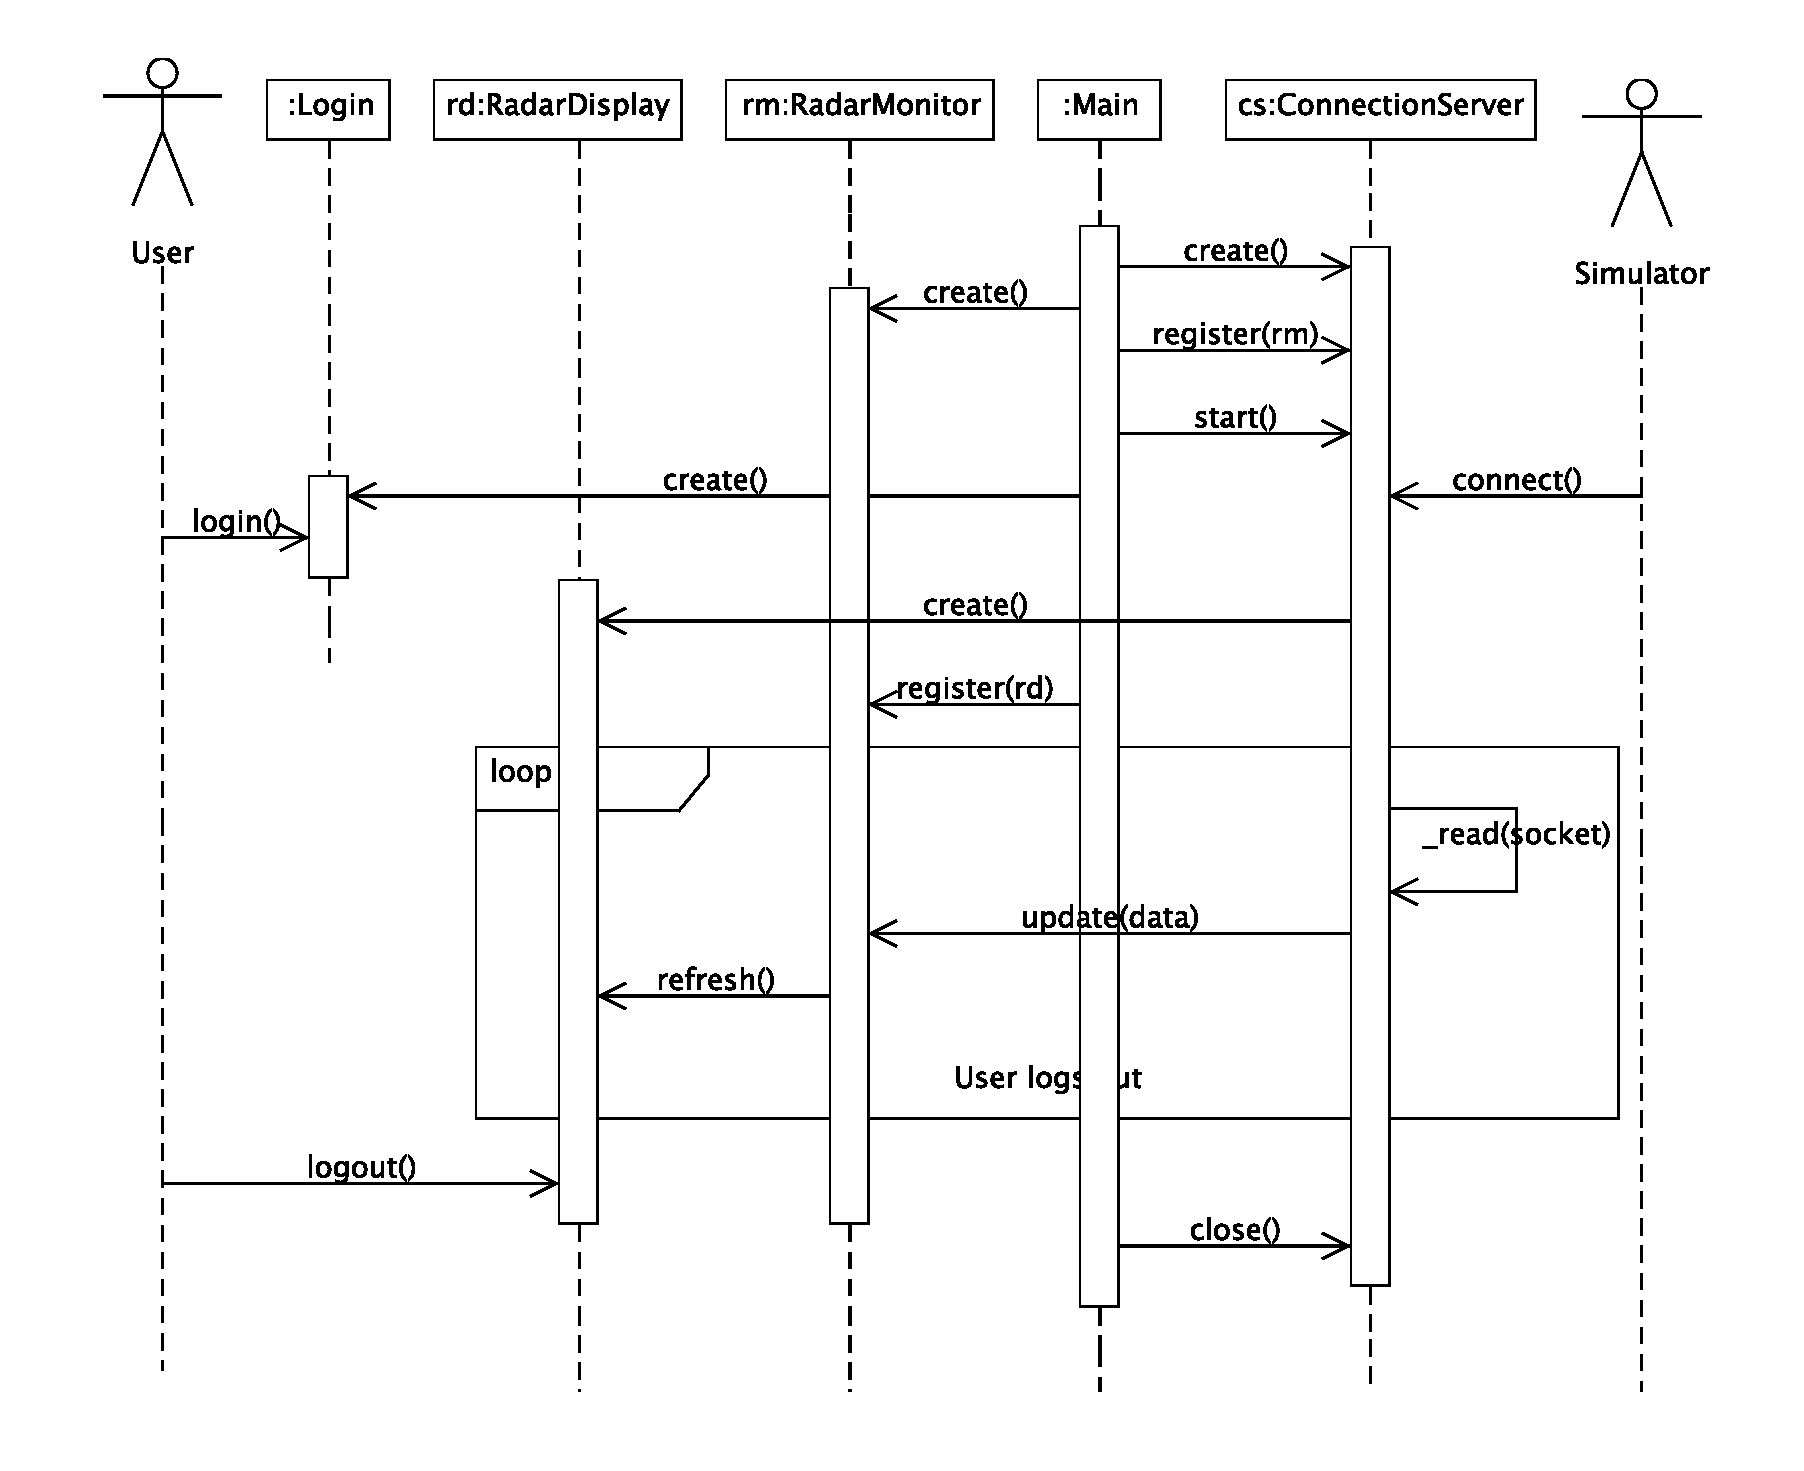
\includegraphics[scale=0.6]{diagrams/vms-sequence-diagram.eps}
\end{figure}

\subparagraph{Operational Contracts for VMS Subsystem:}

\begin{description}
  \item[Operation: create() (target: ConnectionServer)] Pre-conditions: none.\newline
  Post-conditions: instance of ConnectionServer is created.
  \item[Operation: create() (target: RadarMonitor)] Pre-conditions: none.\newline
  Post-conditions: instance of RadarMonitor is created.
  \item[Operation: register(RadarMonitor rm)] Pre-conditions: none.\newline
  Post-conditions: passed RadarMonitor is registered as an observer to ConnectionClient.
  \item[Operation: start()] Pre-conditions: Selector is bound.\newline
  Post-conditions: incoming client connections can be accepted.
  \item[Operation: create() (target: Login)] Pre-conditions: none.\newline
  Post-conditions: instance of Login is created.
  \item[Operation: create() (target: RadarDisplay)] Pre-conditions: none.\newline
  Post-conditions: instance of RadarDisplay is created.
  \item[Operation: register(RadarDisplay rd)] Pre-conditions: none.\newline
  Post-conditions: passed RadarDisplay is registered as an observer to RadarMonitor.
  \item[Operation: read(SocketChannel sc)] Pre-conditions:
  - passed SocketChannel is open and connected.\newline
  - data from client was formatted and encoded correctly.\newline
  Post-conditions: data from client is interpreted as vessel data, and all observers are notified.
  \item[Operation: update(UpdateData data)] Pre-conditions: none.\newline
 Post-conditions: data from client replaces current vessel data.
  \item[Operation: refresh()] Pre-conditions: none.\newline
  Post-conditions: GUI-displayed vessel data corresponds to system vessel data.
  \item[Operation: close()] Pre-conditions: none.\newline
  Post-conditions: SocketChannel and Selector are closed.
\end{description}

\section{Revised Cost Estimation} % Status: Complete

\subsection{Cost Estimates}

\begin{description}
  \item[Simulator program:] \$150, cost to code and implement.
  \item[VMS program:] \$150, cost to code and implement.
  \item[Graphical User Interface:] \$100, cost to design, code, and implement.
  \item[Unit test suite:] \$25, cost to write test cases and perform testing.
  \item[Total Cost:] \$425
\end{description}

\paragraph{Basis} Costs have been calculated based on the amount of man hours spent working on project (at a low approximate labor cost of \$5 an hour), as well as a reduced cost of tools used to produce code, test cases, documentation, and diagrams.
Re-estimation of costs may occur when any of the above artifacts is complete, based on whether the artifact took less time or more time than we originally anticipated.

\subsection{Project Schedule}

\begin{description}
  \item[Simulator program:] 8 hours of coding. Due date: August 1st, 2013.
  \item[VMS program:] 8 hours of coding. Due date: August 1st, 2013.
  \item[Graphical User Interface:] 4 hours of coding. Due date: August 7th, 2013.
  \item[Unit test suite:] 2 hour of testing. Due date: August 9th, 2013.
  \item[Final integration:] 4 hours of implementation. Due date: August 12th, 2013.
\end{description}

\paragraph{Note}
The times listed to complete the Simulator program, VMS program, and Graphical User Interface are estimations of how much time the \emph{remainder} of the coding will take, not accounting for the time that has already been spent on the programs as they currently are.

\subsection{Risk}

	All due dates have been calculated with a buffer zone in mind to account for lack of availability depending on course load. Still, course load is difficult to predict, therefore there is a risk that some of the team members will not be able to produce their assigned artifact in time.

Also, writing test cases in parallel with the rest of the software may slightly delay production, although the reliability of the code will be improved.

All cost estimates and due dates are subject to change.

\break
\listoffigures

\end{document}


